
%\section*{Thesis overview}

	\newcommand{\relevance}{\underline{\textbf{\relevanceTXT}}}
%	\newcommand{\progress}{\underline{\textbf{\progressTXT}}}
	\newcommand{\goal}{\underline{\textbf{\goalTXT}}}
	\newcommand{\scientifictasks}{\underline{\textbf{\scientifictasksTXT}}}
	\newcommand{\scientificnovelty}{\underline{\textbf{\scientificnoveltyTXT}}}
	\newcommand{\importance}{\underline{\textbf{\importanceTXT}}}
%	\newcommand{\methods}{\underline{\textbf{\methodsTXT}}}
	\newcommand{\statements}{\underline{\textbf{\statementsTXT}}}
	\newcommand{\validity}{\underline{\textbf{\validityTXT}}}
	\newcommand{\approbation}{\underline{\textbf{\approbationTXT}}}
	\newcommand{\implementation}{\underline{\textbf{\implementationTXT}}}
%	\newcommand{\contribution}{\underline{\textbf{\contributionTXT}}}
	\newcommand{\refs}{\underline{\textbf{\refsTXT}}}
\chapter*{Synopsis}
\addcontentsline{toc}{chapter}{Synopsis} 
\section*{Thesis overview}

%	\section*{The goal}
%	\section*{Scientific tasks:}
%	\section*{Scientific novelty}
%	\section*{Scientific statements:}
%	\section*{Practical importance}
%	\section*{Reliability and the validity}
%	\section*{Implementation of the obtained results}
%	\section*{Approbation}
%	\section*{Publication}
%	\section*{Author contribution}
%	\section*{The structure}
%	\section*{MAIN CONTENTS OF WORK}


  {\relevance} 
  Quantum informatics is a field of knowledge that combines elements of the photonics and the theory of information. Quantum bits, or qubits, are used as the basic units of quantum information science. Qubit is a system that can be in a superposition state and used to store, calculate and transmit information. One of the promising areas of quantum informatics are a quantum calculations and a quantum memory -- the main components of a quantum computer -- a totally new type of computing device that works on the fundamental principles of quantum mechanics. The transmission of a quantum state at various distances, or quantum teleportation, is another promising application of quantum informatics. The generation of a symmetric bit sequence by the quantum methods, or quantum key distribution (QKD), was formed as a scientific direction in the 80's of the 20th century. This direction is advanced in terms of application. In quantum communication systems (QCS), through the use of quantum states, two or more legitimate users can distribute symmetric bit sequences, which can subsequently be used as keys for encoding information, so that any eavesdropping attempts of the communication channel will be detected by the increased error rate.
  
Differences between physical implementations of QCS from ideal models used in theoretical approaches can be the basis for conducting various types of attacks on equipment used in this systems. It was previously shown that gated single-photon detectors (SPD) of several commercially available QKD systems were vulnerable to attack by the eavesdropper. It is noteworthy that exposure can be carried out even by optical methods. Eavesdropping can be made directly from a quantum channel that connects legitimate users. In practice, optical fiber is most often used as a medium for the transferring of quantum states. Single photons and their properties are usually used for that purposes.
	
This type of attack is called a <<faked-states attack>> (FSA). It is based on the fact that for the detection of photons, a detector based on avalanche photodiodes (APDs) operating in the Geiger mode, or photon counting mode, is used. With this approach, in the absence of additional protective measures, the attacker has the ability to use the powerful constant optical radiation to carry the detector out from the Geiger mode to the linear mode (so-called <<blinding>>) and provoke triggering due to the use of powerful short pulses. Thus, the feasibility of complete control of the single-photon registration node, became critical for QKD protocols, and as a result, leads the eavesdropper to imperceptible obtaining of the full key correlating with that of legitimate users.
	

There are several ways to counter this type of attack, but in practice most of them have not been tested in quantum hacking laboratories. Several countermeasures that were analyzed and investigated have included counterattacks and hacking methods that were not taken into account by the developers of countermeasures.
	
The most effective countermeasure against the well-known types of attacks on detector side is the implementation of a  quite new QKD architecture that is resistant to attacks on measuring equipment (Measurement-Device-Independent, or MDI). With this approach, it is initially assumed that the single-photon registration unit is moved outside the sender and receiver blocks and is completely accessible to the eavesdropper. However, such an approach is characterized by a higher level of complexity of implementing the optical scheme and lower characteristics with respect to QKD systems with a point-to-point topology with a registration node in one of the blocks.
	
One of the promising approaches is the method of quantum communication at subcarrier-wave quantum key distribution (SCW~QKD). Its distinctive feature is the carrying of the quantum channel out to the sidebands generated as a result of modulation. This ensures high resistance to external factors and spectral efficiency, as well as good performance in the ratio of the key formation speed to the distance between the sender and receiver units. However, as part of this type of system for small and medium distances (up to 100~km), single-photon detectors based on the APD are also used, and the resistance to attacks on the measuring equipment of SCW~QKD systems has not been investigated.
	
	
% Обзор, введение в тему, обозначение места данной работы в
% мировых исследованиях и~т.\:п., можно использовать ссылки на~другие
% работы\ifnumequal{\value{bibliosel}}{1}{~\autocite{Gosele1999161}}{}
% (если их~нет, то~в~автореферате
% автоматически пропадёт раздел <<Список литературы>>). Внимание! Ссылки
% на~другие работы в разделе общей характеристики работы можно
% использовать только при использовании \verb!biblatex! (из-за технических
% ограничений \verb!bibtex8!. Это связано с тем, что одна
% и~та~же~характеристика используются и~в~тексте диссертации, и в
% автореферате. В~последнем, согласно ГОСТ, должен присутствовать список
% работ автора по~теме диссертации, а~\verb!bibtex8! не~умеет выводить в одном
% файле два списка литературы).
% При использовании \verb!biblatex! возможно использование исключительно
% в~автореферате подстрочных ссылок
% для других работ командой \verb!\autocite!, а~также цитирование
% собственных работ командой \verb!\cite!. Для этого в~файле
% \verb!Synopsis/setup.tex! необходимо присвоить положительное значение
% счётчику \verb!\setcounter{usefootcite}{1}!.
% 
% Для генерации содержимого титульного листа автореферата, диссертации
% и~презентации используются данные из файла \verb!common/data.tex!. Если,
% например, вы меняете название диссертации, то оно автоматически
% появится в~итоговых файлах после очередного запуска \LaTeX. Согласно
% ГОСТ 7.0.11-2011 <<5.1.1 Титульный лист является первой страницей
% диссертации, служит источником информации, необходимой для обработки и
% поиска документа>>. Наличие логотипа организации на~титульном листе
% упрощает обработку и~поиск, для этого разметите логотип вашей
% организации в папке images в~формате PDF (лучше найти его в векторном
% варианте, чтобы он хорошо смотрелся при печати) под именем
% \verb!logo.pdf!. Настроить размер изображения с логотипом можно
% в~соответствующих местах файлов \verb!title.tex!  отдельно для
% диссертации и автореферата. Если вам логотип не~нужен, то просто
% удалите файл с~логотипом.

% \ifsynopsis
% Этот абзац появляется только в~автореферате.
% Для формирования блоков, которые будут обрабатываться только в~автореферате,
% заведена проверка условия \verb!\!\verb!ifsynopsis!.
% Значение условия задаётся в~основном файле документа (\verb!synopsis.tex! для
% автореферата).
% \else
% Этот абзац появляется только в~диссертации.    ----- условие выполняется как else в обоих случаях (для диссертации и реферата)
% Через проверку условия \verb!\!\verb!ifsynopsis!, задаваемого в~основном файле
% документа (\verb!dissertation.tex! для диссертации), можно сделать новую
% команду, обеспечивающую появление цитаты в~диссертации, но~не~в~автореферате.
% \fi

% {\progress}
% Этот раздел должен быть отдельным структурным элементом по
% ГОСТ, но он, как правило, включается в описание актуальности
% темы. Нужен он отдельным структурынм элемементом или нет ---
% смотрите другие диссертации вашего совета, скорее всего не нужен.

{\goal} of this dissertation is to investigate a feasibility of the secret key eavesdropping by detector side channel attacks of SCW~QKD systems and to develop countermeasure methods.


{\scientifictasks}:
\begin{enumerate}
  \item Investigate vulnerability to blinding of the SPD used in SCW~QKD.  

  \item Estimate the eavesdropper limits in case of successfully controlling detector side. 

  \item Develop an optical scheme for monitoring possible eavesdropping.

  \item Investigate a measurement-device independent QKD protocol based on multi-mode weak coherent states used in SCW~QKD. 
\end{enumerate}


{\scientificnovelty} is specified by the following new results:
\begin{enumerate}
  \item It is experimentally demonstrated the vulnerability of SCW~QKD to faked-state attacks.
  \item For the first time it is shown that the SCW~QKD basic optical scheme provides an advantage and could be updated for monitoring the bright light.
  \item It is proposed and experimentally studied the feasibility of twin-field quantum key distribution based on multi-mode coherent phase-coded states. The detection node is moved away to untrusted relay. The nontrivial interference is obtained. Key rate estimation shows that SCW approach can beat well-known fundamental limits of repeaterless quantum communications (linear bound).
\end{enumerate}

{\statements}
\begin{enumerate}

  \item Single-photon detector based on avalanche photodiode with 100~MHz external gating could be moved out from photon-counting mode by bright light illumination no less than 35 nW. It could be triggered by optical pulses with energy more than 15,4 fJ regardless of their repetition rate.
  \item The frequency conversion of the control signal by phase modulation on the radio frequency mode allows to detect a faked-state attack by monitoring a carrier's frequency.
  \item The use of weak coherent multi-mode states with phase coding makes it possible to implement a protocol that is resistant to control by an illegitimate user of measuring device.
  \item In result of interference of quantum states at sidebands on a symmetrical beam splitter placed in untrusted detection node, the spectral separation of the quantum signal and the signal at the central wavelength occurs with their independent registration in different beamsplitter outputs. 
  %  \item Double distance increasing is performed by using twin-field approach for multi-mode weak coherent phase-coded states. 
  %  \item Показана возможность двукратного увеличения дальности квантовой рассылки ключа на боковых частотах посредством применения недоверенной системы регистрации квантовых состояний. 
 
\end{enumerate}
{\influence} 

Разработанные методы и подход позволили однозначно определить уязвимость коммерчески доступных детекторов компании id Quantique модели id210 к выведению из режима Гейгера оптическими средствами. В связи с чем доказана необходимость применения дополнительных мер защиты от атак на измерительный узел. Предложена схема, позволяющая производить активный мониторинг попыток <<ослепить>> детектор, благодаря использованию особенностей систем квантовой коммуникации на боковых частотах. Результаты внедрены в производство ООО "Кванттелеком". 

%  {\methods} \todo{TO DO} \ldots

%%%%%	{\defpositions}
%%%%%	\begin{enumerate}
%%%%%  \item Использование коммерческих детекторов одиночных фотонов на основе лавинных фотодиодов в режиме Гейгера модели id210 с частотой стробирования 100 МГц  требует применения дополнительных средств защиты от атаки с выведением из режима Гейгера при помощи коротких оптических импульсов с энергией не менее 15,4 фДж и при постоянном уровне оптической засветки средним уровнем мощности излучения не менее 35 нВт.  
%%%%%  \item Измерение величины оптического излучения на несущей частоте, отраженного от оптического фильтра, при помощи мониторного фотодиода в приемном блоке системы квантовой коммуникации на боковых частотах в диапазоне от 7 нВт до 2,93 мкВт с применением дополнительных мер в виде пассивного оптического аттенюатора номиналом 10 дБ для его защиты позволяет противостоять атаке с выведением детектора одиночных фотонов из режима Гейгера и навязыванием ключа нелегитимным пользователем. 
%%%%%  \item Метод квантовой коммуникации на боковых частотах позволяет реализовывать протокол, устойчивый к контролю нелегитимным пользователем измерительного оборудования. 
%%%%%  \item В результате интерференции квантового фазомодулированного сигнала на боковых частотах на симметричном светоделителе в схеме квантовой рассылки ключа с узлом регистрации, независящим от легитимного пользователя, происходит спектральное разделение квантового сигнала и сигнала на центральной длине волны с их независимой регистрацией в разных плечах светоделителя. 
%%%%%%%  \item Показана возможность двукратного увеличения дальности квантовой рассылки ключа на боковых частотах посредством применения недоверенной системы регистрации квантовых состояний. 
%%%%%%%%\end{enumerate}
% В папке Documents можно ознакомиться в решением совета из Томского ГУ
% в~файле \verb+Def_positions.pdf+, где обоснованно даются рекомендации
% по~формулировкам защищаемых положений.




{\reliability} полученных результатов обеспечивается применением утверждённых методик проведений экспериментальных исследований и аттестованного оборудование. Математическое моделирование и обработка данных, полученных в результате экспериментов, осуществлялось с использованием пакетов прикладных программ MathCad и Excel. Результаты находятся в соответствии с результатами, полученными другими авторами.


{\probation}
Основные результаты работы докладывались~на:
%перечисление основных конференций, симпозиумов и~т.\:п. 
\begin{enumerate}
	\item ICQOQI 2019, Минск, Беларусь, 13 - 17 мая 2019
	\item XLVIII научная и учебно-методическая конференция Университета~ИТМО, Санкт-Петербург, Россия, 29 января - 1 февраля 2019
	\item QCrypt 2018, Шанхай, Китай, 27 - 31 августа 2018
	\item 18th International Conference on Laser Optics ICLO 2018, Санкт-Петербург, Россия, 4 - 8 июня 2018
	\item VII Всероссийский конгресс молодых ученых, Санкт-Петербург, Россия, 17 - 20 апреля 2018
	\item XLVII научная и учебно-методическая конференция Университета ИТМО, Санкт-Петербург, Россия, 30 января - 2 февраля 2018
\end{enumerate}

% {\contribution} Автор принимал активное участие \todo{TO DO} \ldots

%\publications\ Основные результаты по теме диссертации изложены в ХХ печатных изданиях~\cite{Sokolov,Gaidaenko,Lermontov,Management},
%Х из которых изданы в журналах, рекомендованных ВАК~\cite{Sokolov,Gaidaenko},
%ХХ --- в тезисах докладов~\cite{Lermontov,Management}.

\ifnumequal{\value{bibliosel}}{0}{% Встроенная реализация с загрузкой файла через движок bibtex8
    \publications\ Основные результаты по теме диссертации изложены в XX печатных изданиях,
    X из которых изданы в журналах, рекомендованных ВАК,
    X "--- в тезисах докладов.%
}{% Реализация пакетом biblatex через движок biber
%Сделана отдельная секция, чтобы не отображались в списке цитированных материалов
    \begin{refsection}[vak,wos,scopus,papers,conf]% Подсчет и нумерация авторских работ. Засчитываются только те, которые были прописаны внутри \nocite{}.
        %Чтобы сменить порядок разделов в сгрупированном списке литературы необходимо перетасовать следующие три строчки, а также команды в разделе \newcommand*{\insertbiblioauthorgrouped} в файле biblio/biblatex.tex
        \printbibliography[heading=countauthorvak, env=countauthorvak, keyword=biblioauthorvak, section=1]%
        \printbibliography[heading=countauthorwos,env=countauthorwos, keyword=biblioauthorwos, section=1]%
        \printbibliography[heading=countauthorscopus,env=countauthorscopus, keyword=biblioauthorscopus, section=1]%
	\printbibliography[heading=countauthorconf, env=countauthorconf, keyword=biblioauthorconf, section=1]%
        \printbibliography[heading=countauthorothers, env=countauthorothers, keyword=biblioauthorothers, section=1]%
        \printbibliography[heading=countauthor, env=countauthor, keyword=biblioauthor, section=1]%
        \nocite{%Порядок перечисления в этом блоке определяет порядок вывода в списке публикаций автора
                JOT,Chistyakov_2016,%
		Chistiakov:19,%
		scbib1,%
                confbib1,confbib2,%
                bib1,bib2,%
        }%
	\publications\ Основные результаты по теме диссертации изложены в 13 печатных изданиях. 10 из которых изданы в журналах, рекомендованных ВАК, 3 в тезисах докладов. 
	
	\section*{Работы автора по теме диссертации}
{Статьи в журналах, рекомендованных ВАК: }
\begin{enumerate}\addtolength{\itemsep}{-0.5\baselineskip}
\renewcommand{\labelenumi}{[\theenumi]}
\item Vladimir Chistiakov, Anqi Huang, Vladimir Egorov, and Vadim Makarov, Controlling single-photon detector ID210 with bright light, Opt. Express 27, 32253-32262 (2019)
\\
\item Чистяков В.В., Гайдаш А.А., Козубов А.В., Глейм А.В. Исследование интерференции слабых когерентных многомодовых состояний для задач квантовой коммуникации с недоверенным приемным узлом // Научно-технический вестник информационных технологий, механики и оптики. 2019. Т. 19. № 6. doi: 10.17586/2226-1494-2019-19-6
\\
\item    Gleim A.V., Egorov V.I., Nazarov Y.V., Smirnov S.V., Chistyakov V.V., Bannik O.I., Anisimov A.A., Kynev S.M., Ivanova A.E., Collins R.J., Kozlov S.A., Buller G. Secure polarization-independent subcarrier quantum key distribution in optical fiber channel using BB84 protocol with a strong reference//Optics express, IET - 2016, Vol. 24, No. 3, pp. 2619-2633
\\
\item  Глейм А.В., Егоров В.И., Чистяков В.В., Смирнов С.В., Банник О.И., Булдаков Н.В., Гайдаш А.А., Козубов А.В., Васильев А.Б., Кынев С.М., Хоружников С.Э., Козлов С.А., Васильев В.Н. Квантовая коммуникация на боковых частотах со скоростью 1 Мбит/с в городской сети // Оптический журнал -2017. - Т. 84. - № 6. - С. 3-9
\\
\item  Chistyakov V.V., Kynev S.M, Smirnov S.V., Nazarov Y.V., Gleim A.V. Achieving high visibility in subcarrier wave quantum key distribution system // Journal of Physics: Conference Series, IET - 2016, Vol. 735, No. 1, pp. 012085
\\
\item V. V. Chistyakov, A. V. Gleim, V. I. Egorov, Yu. V. Nazarov. Implementation of multiplexing in a subcarrier-wave quantum cryptography system // Journal of Physics: Conference Series - 2014  vol. 541,  pp. 012078
\\
\item   Kynev S.M., Chistyakov V.V., Smirnov S.V., Volkova K.P., Egorov V.I., Gleim A.V. Free-space subcarrier wave quantum communication // Journal of Physics: Conference Series - 2017, Vol. 917, No. 5, pp. 052003
\\

\item    Gleim A.V., Nazarov Y.V., Egorov V.I., Smirnov S.V., Bannik O.I., Chistyakov V.V., Kynev S.M., Anisimov A.A., Kozlov S.A., Vasil'ev V.N. Subcarrier Wave Quantum Key Distribution in Telecommunication Network with Bitrate 800 kbit/s//EPJ Web of Conferences, IET - 2015, Vol. 103, pp. 10005
\\
\item    Gleim A.V., Egorov V.I., Nazarov Y.V., Smirnov S.V., Chistyakov V.V., Bannik O.I., Anisimov A.A., Kynev S.M., Collins R.J., Kozlov S.A., Buller G.S. Polarization insensitive 100 MHz clock subcarrier quantum key distribution over a 45 dB loss optical fiber channel // Conference on Lasers and Electro-Optics, CLEO 2015, IET - 2015, pp. 7182997
\\
\item Gaidash A.A., Kozubov A.V., Chistyakov V.V., Miroshnichenko G.P., Egorov V.I., Gleim A.V. Security conditions for sub-carrier wave quantum key distribution protocol in errorless channel // Journal of Physics: Conference Series - 2017, Vol. 917, No. 6, pp. 062014
\\
%\item  Gleim A.V., Chistyakov V.V., Bannik O.I., Egorov V.I., Buldakov N.V., Vasilev A.B., Gaidash A.A., Kozubov A.V., Smirnov S.V., Kynev S.M., Khoruzhnikov S.E., Kozlov S.A., Vasil'ev V.N. Sideband quantum communication at 1 Mbit/s on a metropolitan area network // Journal of Optical Technology - 2017, Vol. 84, No. 6, pp. 362-36
\\

\end{enumerate}
\noindent{ Другие публикации: }
\begin{enumerate}\addtolength{\itemsep}{-0.5\baselineskip}
\renewcommand{\labelenumi}{[\theenumi]}
\setcounter{enumi}{9}
\item   Чистяков В.В., Кынев С.М., Смирнов С.В., Назаров Ю.В., Глейм А.В. Обеспечение высокой видности в системе квантовой криптографии на боковых частотах // Сборник трудов IX международной конференции молодых ученых и специалистов «Оптика – 2015», с. 658-660
\\
\item Глейм А.В., Назаров Ю.В., Егоров В.И., Чистяков В.В, Смирнов С.В., Банник О.И., Кынев С.М., Иванова А.Е., Дубровская В.Д., Тарасов М.Г., Булдаков Н.В., Кузьмина Т.Б., Чивилихин С.А., Анисимов А.А., Рощупкин С.В., Рогачёв К.С., Хоружников С.Э., Козлов С.А., Васильев В.Н. Создание квантовой сети университета ИТМО //Сборник трудов VIII международной конференции «Фундаментальные проблемы оптики – 2014». Санкт-Петербург, 20-24 октября ,2014, С.3-4,  541 с. 
\\
\item А.В. Глейм, В.И.Егоров, А.А. Анисимов, Ю.В. Назаров, С.М. Кынев, А.В. Рупасов, В.В. Чистяков, А.А.Гайдаш, М.А. Смирнов, С.А. Чивилихин, С.А. Козлов Квантовая рассылка криптографического ключа по оптическому волокну телекоммуникационного стандарта на расстояние 200 км со скоростью 0.18 кбит/с // Cборник трудов III Всероссийская конференция по фотонике и информационной оптике Москва, НИЯУ МИФИ, 2014 с. 17-19
\\


\end{enumerate}

	
%	\setcounter{citeauthorscwostot}{\value{citeauthorscopus}} % вместе setcounter и addtocounter добавляют пробел между словами. По-этому они так раскиданы.
%        в~\arabic{citeauthor}~печатных изданиях,
%	\addtocounter{citeauthorscwostot}{\value{citeauthorwos}}
%	\arabic{citeauthorvak} из которых изданы в журналах, рекомендованных ВАК\sloppy
%	\ifnum \value{citeauthorscwostot}>0
%	, \arabic{citeauthorscwostot} "--- в~периодических научных журналах, индексируемых Web of Science и Scopus\sloppy
%	\fi
%	\ifnum \value{citeauthorconf}>0
%	, \arabic{citeauthorconf} "--- в~тезисах докладов.
%	\else
%	.
%	\fi
%    \end{refsection}
%    \begin{refsection}[vak,wos,scopus,papers,conf]%Блок, позволяющий отобрать из всех работ автора наиболее значимые, и только их вывести в автореферате, но считать в блоке выше общее число работ
%        \printbibliography[heading=countauthorvak, env=countauthorvak, keyword=biblioauthorvak, section=2]%
%        \printbibliography[heading=countauthorwos, env=countauthorwos, keyword=biblioauthorwos, section=2]%
 %       \printbibliography[heading=countauthorscopus, env=countauthorscopus, keyword=biblioauthorscopus, section=2]%
  %      \printbibliography[heading=countauthorothers, env=countauthorothers, keyword=biblioauthorothers, section=2]%
  %      \printbibliography[heading=countauthorconf, env=countauthorconf, keyword=biblioauthorconf, section=2]%
   %     \printbibliography[heading=countauthor, env=countauthor, keyword=biblioauthor, section=2]%
        
    %    \nocite{Chistyakov_2016}%vak
    %    \nocite{Gleim:15}
    %    \nocite{Gleim:16}
    %    \nocite{Gleĭm:17}
        
     %   \nocite{bib1}%other
     %   \nocite{confbib1}%conf
   \end{refsection}
}
% При использовании пакета \verb!biblatex! для автоматического подсчёта
% количества публикаций автора по теме диссертации, необходимо
% их~здесь перечислить с использованием команды \verb!\nocite!.
 % Характеристика работы по структуре во введении и в автореферате не отличается (ГОСТ Р 7.0.11, пункты 5.3.1 и 9.2.1), потому её загружаем из одного и того же внешнего файла, предварительно задав форму выделения некоторым параметрам

%Диссертационная работа была выполнена при поддержке грантов ...

%\underline{\textbf{Объем и структура работы.}} Диссертация состоит из~введения,
%четырех глав, заключения и~приложения. Полный объем диссертации
%\textbf{ХХХ}~страниц текста с~\textbf{ХХ}~рисунками и~5~таблицами. Список
%литературы содержит \textbf{ХХX}~наименование.

 \section*{Main contents of work}
In the \underline{\textbf{introduction}} we explain the relevance of research carried out in the thesis, formulate the goal, set the tasks, and state the scientific novelty and practical significance of the work.

The \underline{\textbf{first chapter}} is a review, where main currently known methods for detecting single photons in quantum communication systems are considered. We analyze and compare various types of photon detectors, and justify the choice of a single photon detector (SPD) (based on avalanche breakdown) studied in this work. We then consider possible attacks by a potential eavesdropper on the measuring equipment, as well as known countermeasures against this class of attacks.

%  картинку можно добавить так:
% \begin{figure}[ht]
%   \centering
%   
\includegraphics [scale=0.27] {latex}
%   \caption{Подпись к картинке.}
 %  \label{fig:latex}
% \end{figure}

% Формулы в строку без номера добавляются так:
% \[
%   \lambda_{T_s} = K_x\frac{d{x}}{d{T_s}}, \qquad
%   \lambda_{q_s} = K_x\frac{d{x}}{d{q_s}},
% \]

The \underline{\textbf{second chapter}} is devoted to studying an SPD based on avalanche breakdown in a photodiode (an APD), which is used as measuring device for registering the result of quantum states interference in a subcarrier-wave (SCW) QKD system. This type of SPDs is usually used for QKD over mid-range distances of up to 100 ~ km with losses in communication lines less than 15~dB.

Main advantages of this SPD are the following:
\begin{enumerate}
	\item High frequency trigger pulses - up to 100~MHz.
	\item Ability to supply strobe pulses from an external device (External gating mode).
	\item Wide range of operation window (gate) width - from 0.5~ns to 25~ns.
	\item Ability to set a delay between the gate and the strobe pulse (Trigger delay) up to 10~ns with high time resolution - 10~ps.
	\item <<Dead time>> can be adjusted in a wide range - from 0.1~μs to 100~μs.
	\item Tunable quantum efficiency in the range from 5~\% to 25~\% with 2.5~\% step.
	\item Semiconductor APD structure - InGaAs/InP.
	\item Relatively low level of dark counting with given parameters of quantum efficiency.
\end{enumerate}

In course of the study, in order to emulate realistic conditions for the eavesdropper during their attack one the APD, as on a measuring device in the SCW QKD system, the detector was considered as a <<black box>>. Thus, it was not opened and no manipulations were made with its internal boards or microcircuits. All detector settings were in accordance with its standard mode of operation in the SCW QKD system.

In order to successfully carry out a faked-states attack (FSA), an eavesdropper needs to manipulate the detector by forcing it to clicks (and not to click) at the desired time instances. It is assumed that the type of measuring device used is known to the eavesdropper, but they have no direct access to it. In that case the model is limited by a possibility of influencing the detector only by optical methods, directly from the quantum channel.

It is known that when an APD is operating in a linear mode, incident optical power raises the photocurrent. Therefore, if the optical power remains constant, and we apply reverse bias voltage $-V_{bias}$ in the presence of a resistor, which quenches the avalanche in the circuit, the voltage drop will increase on the resistor and decrease on the APD. The idea of FSA lies in switching the APD from the Geiger mode to linear mode, or <"blinding">> it. In other words, its operating mode is shifted relative to the breakdown voltage. With this approach, even additional $V_{gate}$ pulses become insufficient, and the diode always remains in the mode of linear photocurrent dependence on the incident optical power.  

Nevertheless, in linear mode, it remains possible to exceed the threshold value of the photocurrent $I_{det}$ and generate a detector response.

Thus, the technique of switching the detector from the photon-counting (Geiger) mode to the linear mode for carrying out the FSA can be easily formalized. An experimental study SPD vulnerability to this type of attack is carried out in three stages, as shown in figure \ref{fig:Method_2.3}:
%
 \begin{figure}[ht] 
  \centering
  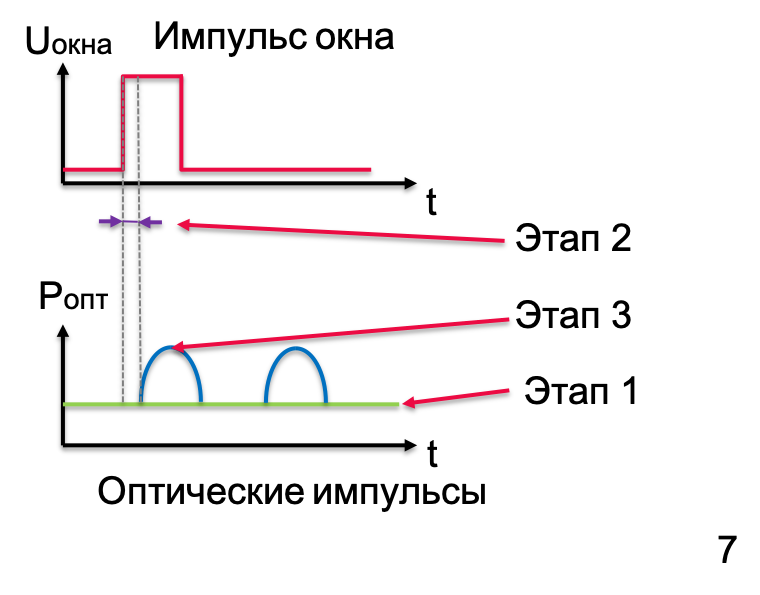
\includegraphics[scale=0.5]{Method_2.3.eps}
  \caption{Blinding methods}
  \label{fig:Method_2.3}
\end{figure}
%
 \begin{enumerate}
	\item Determining constant optical power level sufficient to switch the detector from the Geiger mode into linear mode.
	\item Optical pulse adjustment for the SPD gate
	\item Click probability dependence on photon energy in the trigger pulse.
\end{enumerate}
%
As a result of experimental study detector click probabilities were obtained (fig. \ref{fig:Probability_vs_Energy}). 

\begin{figure}[ht]
  \centering
  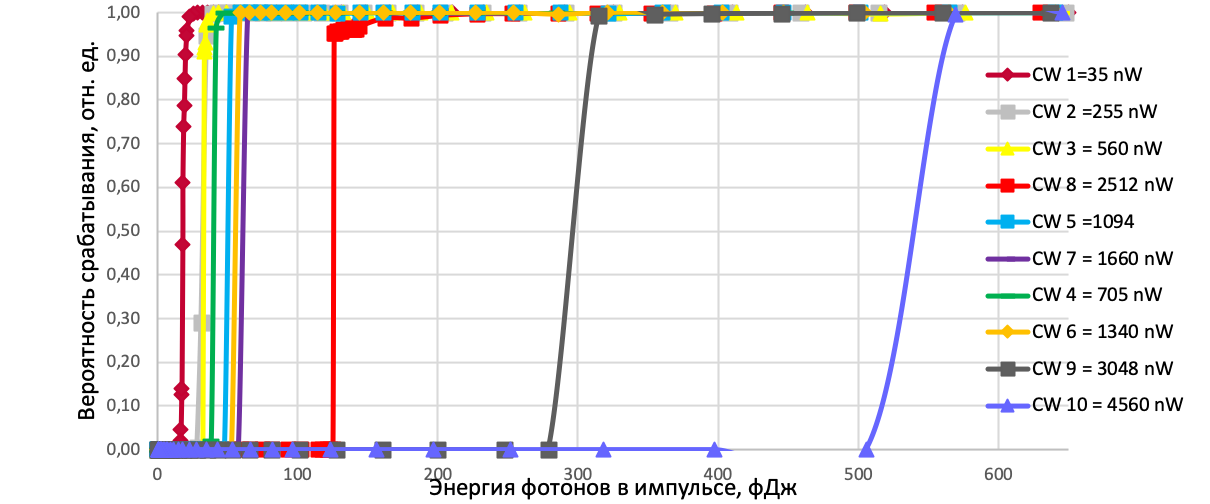
\includegraphics[scale=0.5]{Probability_vs_Energy.png}
  \caption{Detector click probability as a function of trigger pulse energy}
  \label{fig:Probability_vs_Energy}
\end{figure}


Thus, it has been shown that using SPD based on APD operating in Geiger mode (id210) with 100 MHz gating frequency requires additional means of protection against an FSA attack, which constitutes in switching the APD from Geiger mode to linear mode by short optical pulses with energy of at least 15.4~fJ and a constant level of optical illumination with an average radiation power level at least 35~nW. 

A study of FSA on SCW~QKD systems is conducted in the \underline{\textbf{third chapter}}. The applicability limits of this attack are estimated taking into account component parameters in a realistic SCW QKD receiver unit. To uncover the eavesdropper's attempts to carry out the attack (as described above), it is proposed to measure the intensity of the central optical mode. In SCW QKD, the central mode is reflected from a narrow-band filter based on fiber Bragg grating. In order measure the carrier power, a fiber optic circulator can be installed in the circuit. All radiation that passes through the phase modulators and enters the first port of the circulator is directed into the second port, to the optical filter. The reflected central mode is then sent to the third port of the circulator. In order to measure its power, which, as shown in the section, is exptected to be about 700 ~ nW, it is proposed to use a watchdog photodiode. If the eavesdropper has the opportunity to select the intensity on the central mode, it is obvious that the photodiode installed at the output from the 3rd port can also be controlled (blinded) by optical methods. In order to avoid this, we propose using a fiber optic mirror, for example a widely available Faraday mirror, and a fixed passive optical attenuator. The monitor photodiode itself can then be is proposed to be installed at the 4th port of the circulator. Thus, the radiation with the central mode arrives at the 3rd port, passes the attenuator in the forward direction, is reflected from the fiber mirror, passes the attenuator in the opposite direction, and arrives at the 4th port where, the protected monitor photodiode is installed.       
 \begin{figure}[ht]
  \centering
  \includegraphics[scale=0.25]{scw-setup_Countermeasure.pdf}
  \caption{Eavesdropper model for FSA implementation}
  \label{fig:countermeasure}
\end{figure}


Figure \ref{fig:Watchdog_photodiode} shows two dependencies: a lower limit of  optical power required to switch the APD from the Geiger mode (minimal required for a successful FSA), and an upper limit of optical power, calculated fror the SCW system parameters and the maximum optical power of control pulses. According to the calcuation, the minimum level is 0.7 ~ μW, and the maximum is around 300 ~ μW, within the framework of this study.  In practice, however, it is limited by threshold value of the APD inside the SPD at which the current becomes too large and the diode burns out, disrupting the whole device. Typical values are tens of milliwatts.
 
Based on these dependencies we can estimate the loss in the fixed attenuator that will be sufficient to protect the monitor photodiode from exposure to light, and additional measures will not be required to expand the dynamic range of sensitivity to the input optical power in the direction of increase, since at optical powers below few nanowatts the measurement error becomes quite high.

Thus, the attenuation value of 10~dB is sufficient, since the reflected central optical mode at the output from the 3rd port of the circulator passes through the attenuating element for the first time, and then, after reflection from the mirror, once more. The resulting attenuation by 20~dB, or 100 times, will reduce the minimum power level at the central frequency, which is enough to remove the detector from the photon counting mode, to a value of the order of 7~nW, which satisfies the requirements described above. The maximum level (within the framework of this researc) will then decrease to about 3~μW.


 \begin{figure}[ht]
  \centering
  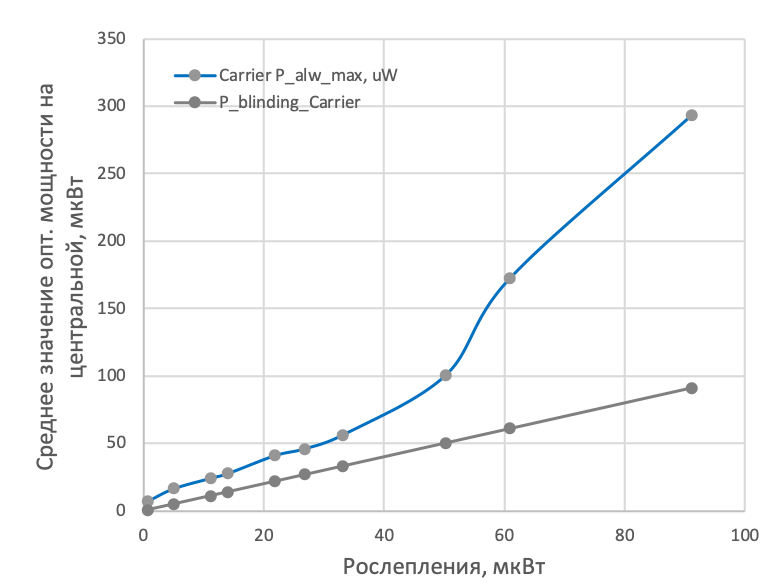
\includegraphics[scale=0.5]{images/Watchdog_photodiode.png}
  \caption{Optical power on monitoring photodiode}
  \label{fig:Watchdog_photodiode}
\end{figure}


In the third chapter we demonstrate how one can protect from FSA in the receiving unit of SCW QKD system by monitoring optical radiation at the carrier frequency, using a monitor photodiode in the range from 7~nW to 2.93~μW and additional countermeasures in the form of a passive optical attenuator with 10 dB loss.

% Можно сослаться на свои работы в автореферате. Для этого в файле
% \verb!Synopsis/setup.tex! необходимо присвоить положительное значение
% счётчику \verb!\setcounter{usefootcite}{1}!. В таком случае ссылки на
% работы других авторов будут подстрочными.
% \ifnumgreater{\value{usefootcite}}{0}{
% Изложенные в третьей главе результаты опубликованы в~\cite{vakbib1, vakbib2}.
% }{}
% Использование подстрочных ссылок внутри таблиц может вызывать проблемы.

 The \underline{\textbf{fourth chapter}} describes the coherent states that are widely used in QCS, because attenuated lasers are widely used as light sources in QKD.
 
  A distinctive feature of SCW QKD systems is the generation of multimode coherent states at different optical modes, depending on the frequency of the modulating signal, as shown in figure \ref{fig:multimodes}. 

 \begin{figure}[ht]
  \centering
  \includegraphics[scale=0.4]{Modes_rus.pdf}
  \caption{Sidebands generation scheme}
  \label{fig:multimodes}
\end{figure}


Let us define these states as follows. Input (unmodulated) state at sender (Alice) and receiver (Bob) sides (denoted as $A$ or $B$) are considered as $|\sqrt{\mu_0}\rangle_0\otimes|\mathrm{vac}\rangle_{SB}$, where $|\mathrm{vac}\rangle_{SB}$ is the sidebands vacuum state and $|\sqrt{\mu_0}\rangle_0$ is a carrier coherent state with an amplitude (mean photon number per pulse) $\mu_0$. The carrier is formed by coherent light beam at a frequency $\omega$. Carrier phase is supposed to be reference, and other phase shifts are defined with respect to it. An electro-optical phase modulator (with modulating frequency $\Omega$ and phase shift $\varphi_A$ or $\varphi_B$) distributes energy fractions between interacting modes. Hence, extra frequencies $\omega_k=\omega+k\Omega$ are observed in the spectrum of the optical signal after the modulator. Considering our case with $2S$ sidebands so number of modes $k$ is limited by $-S\le k\le S$), so the phase modulator's output is the coherent multimode state: 
%
\begin{equation}\label{phi}
|\psi_0(\varphi_j)\rangle = \bigotimes_{k=-S}^S|{\alpha_k(\varphi_j)}\rangle_k,
\end{equation}
%
where $j$ is  $A$ or $B$ (for Alice or Bob), and the signal amplitude becomes as follows: 
%
\begin{equation}\label{alpha}
\alpha_k(\varphi_j)=\sqrt{\mu_0}d^S_{0k}(\beta)e^{i\varphi_jk},
\end{equation}
%
where $d^S_{nk}(\beta)$ is d-Wigner function from the quantum theory of angular momentum  %\cite{varshalovich1988quantum}
, $\beta$ defines by modulation index $m$, that could be noted (without dispersion effects) as: 
%
\begin{equation}\label{betam}
\cos{({\beta})}=1-\frac{1}{2}{\left(\frac{m}{S+0.5}\right)^2},
\end{equation}
where $S$ is the number of interacting modes that is taken very large.

After adjusting the relative phase $\phi_0$ of two optical signals in different arms, the interference on the second beam splitter ($BS2$) is observed. Quantum states on the ($BS2$) outputs are described in~\ref{states}. This relative phase should be adjusted to $\phi_0\approx0$. Then, if the phase difference of modulating radio frequency signals of Alice and Bob modules is ($\Delta\varphi=0$), full multi-mode spectrum goes to the first output of $BS2$, otherwise, even modes with the central one ($k = 0$ mode) go to the same output, and odd modes go to the second output. In case of $\Delta\varphi=0$, the spectrum division of carrier and sidebands is necessary, because the latter contains the quantum information for the key. It should be noted that due to low $m$ a significant contribution to the multimode states is made only by the first pair. The case where $\Delta\varphi=\pi$ is nontrivial. The multi-mode states are divided on $BS2$, and even modes, along with the central one ($k = 0$ mode), go to the first output, while the odds modes (only first pair is significant) go to the second output, as explained in fig. \ref{fig:Interference_result}. Thus, it is possible to abandon spectral separation using an optical filter in one of the output arms of the untrusted measurement unit. An indicator of good phase adjustment of the optical pulses is a constant high level at the carrier frequency in the first output (on $D2$).  


\begin{figure}[ht]
 \centering
  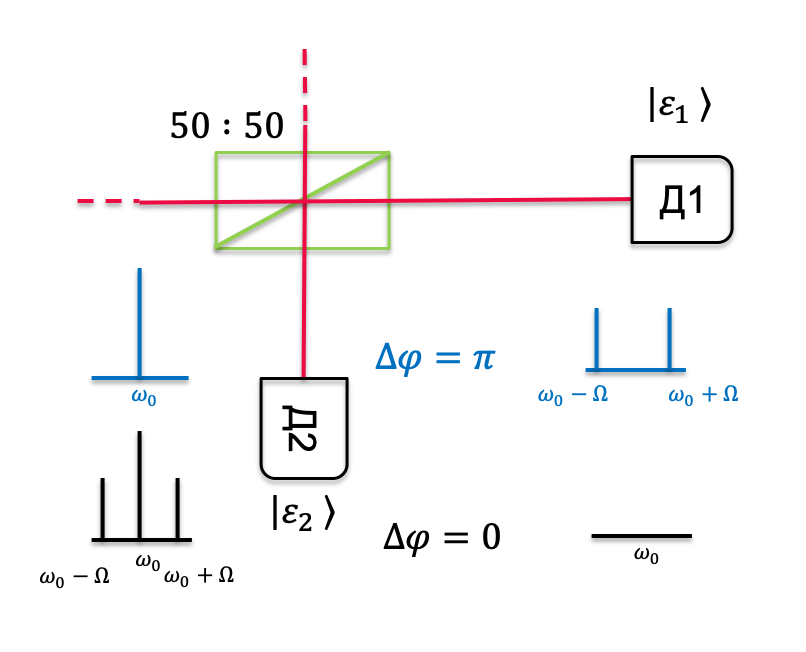
\includegraphics[scale=0.5]{Interference_result.png}
  \caption{Interference of multi-mode weak coherent states}
  \label{fig:Interference_result}
\end{figure}

 
The fourth chapter shows that SCW QKD method allows to implement a measurement-device independent protocol.

QKD protocol scheme using multimode coherent states with an untrusted measuring node is shown in (Fig. \ref{fig:Protocol}). For simplicity, we give an example using only two phase states according to  B92 protocol. Alice randomly choses one phase state from two possible options: <<$0$>> or <<$\pi$>>. Bob, regardless of Alice, also randomly choses one of two phase states. As a result of the interference of multimode coherent states, 4 different cases can be observed, depending on the phase difference chosen by Alice and Bob. In this case, spectral separation will occur on an untrusted detection node, so that the sidebands will arrive at $D1$ and $D2$. At the same time, an eavesdropper has full access to an untrusted measuring node and can record for themselves the announced detector clicks. Let us suppose that we are only interested in the case when the phase difference between $A$ and $B$ is $\pi$. The advantage of this case is that, due to spectral separation during interference, only the sidebands (and not the carrier) will always go into $D1$ arm. It means that an optical filter can be excluded from this arm. This approach is beneficial because matching it with the filter in the other output, $D2$, is a rather difficult engineering task. Thus, during sifting, only bits that correspond to samples on $D1$ remain, and for achieving the correlation between Alice's and Bob's bits, the latter must inverse his information to the opposite (i.e. to perform the so-called <<bitflip>>).

\begin{figure}[ht]
 \centering
  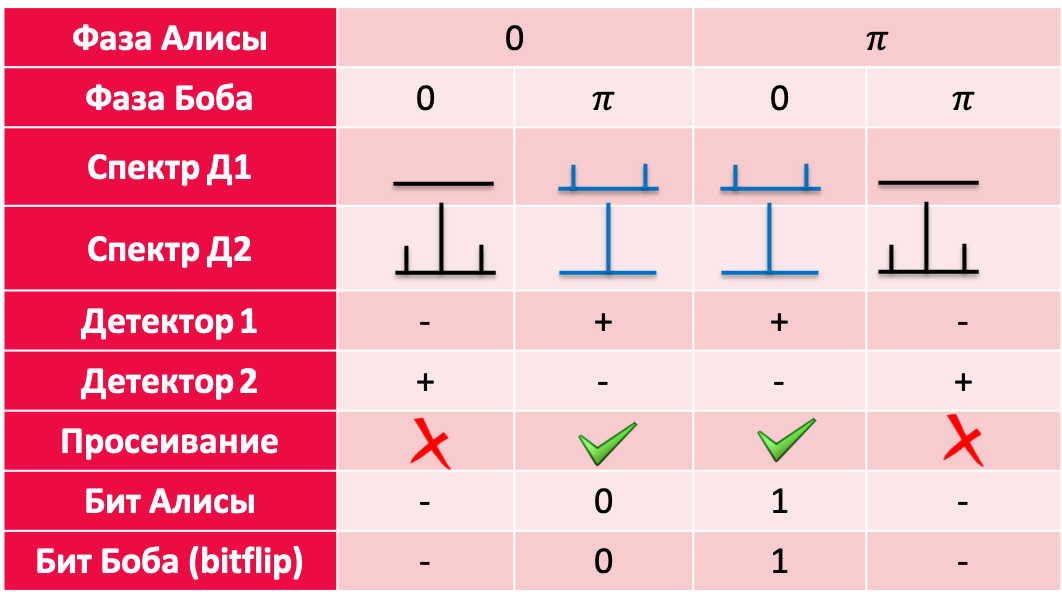
\includegraphics[scale=0.5]{Protocol.png}
  \caption{Протокол}
  \label{fig:Protocol}
\end{figure}
 
In the \underline{\textbf{fifth chapter}} we experimentally study the result of interference of a quantum signal at phase-coded sidebands on a symmetrical beam splitter in a QKD scheme with an untrusted measuring node. Spectral separation of the quantum signal and the carrier with their independent registration at different outputs of the beam splitter is observed. 
  
Our experimental setup is shown in \ref{fig:RF_sin}. For simplicity, only one light source is used, the output of which is shared using a 50:50 $BS1$ beam splitter. This approach allows us to simulate the case when Alice and Bob have well-correlated light sources. In this experiment, a distributed feedback laser (TTX1994 Neophotonics) is used as L1. Its main features are a very narrow spectral linewidth, lower than 100~kHz, and a wide range of wavelength tuning (from 1530~nm to 1565.5~nm) with high accuracy (20~pm). Its output power was 10~mW. However, this value depends on the depth of the dynamic range of the variable optical attenuator VOA and the total losses introduced by Alice or Bob components, since the resulting signal power at the sidebands should not exceed 2.56~pW, corresponding to the average number of photons per pulse 0.2 at 100~MHz repetition rate and wavelength 1550 nm.

Due to high resonator sensitivity of the laser source with distributed feedback (DFB), it necessary to protect it from reflections and scattering of optical signals. A fiber isolator (I) based on the Faraday effect with an isolation value higher than 50~dB is used in the optical scheme. To use the system in single-photon mode, a VOA with a sufficiently small tuning step of 0.05 dB and a large dynamic range of 60~dB is used.

  

  \begin{figure}[ht]
  \centering
  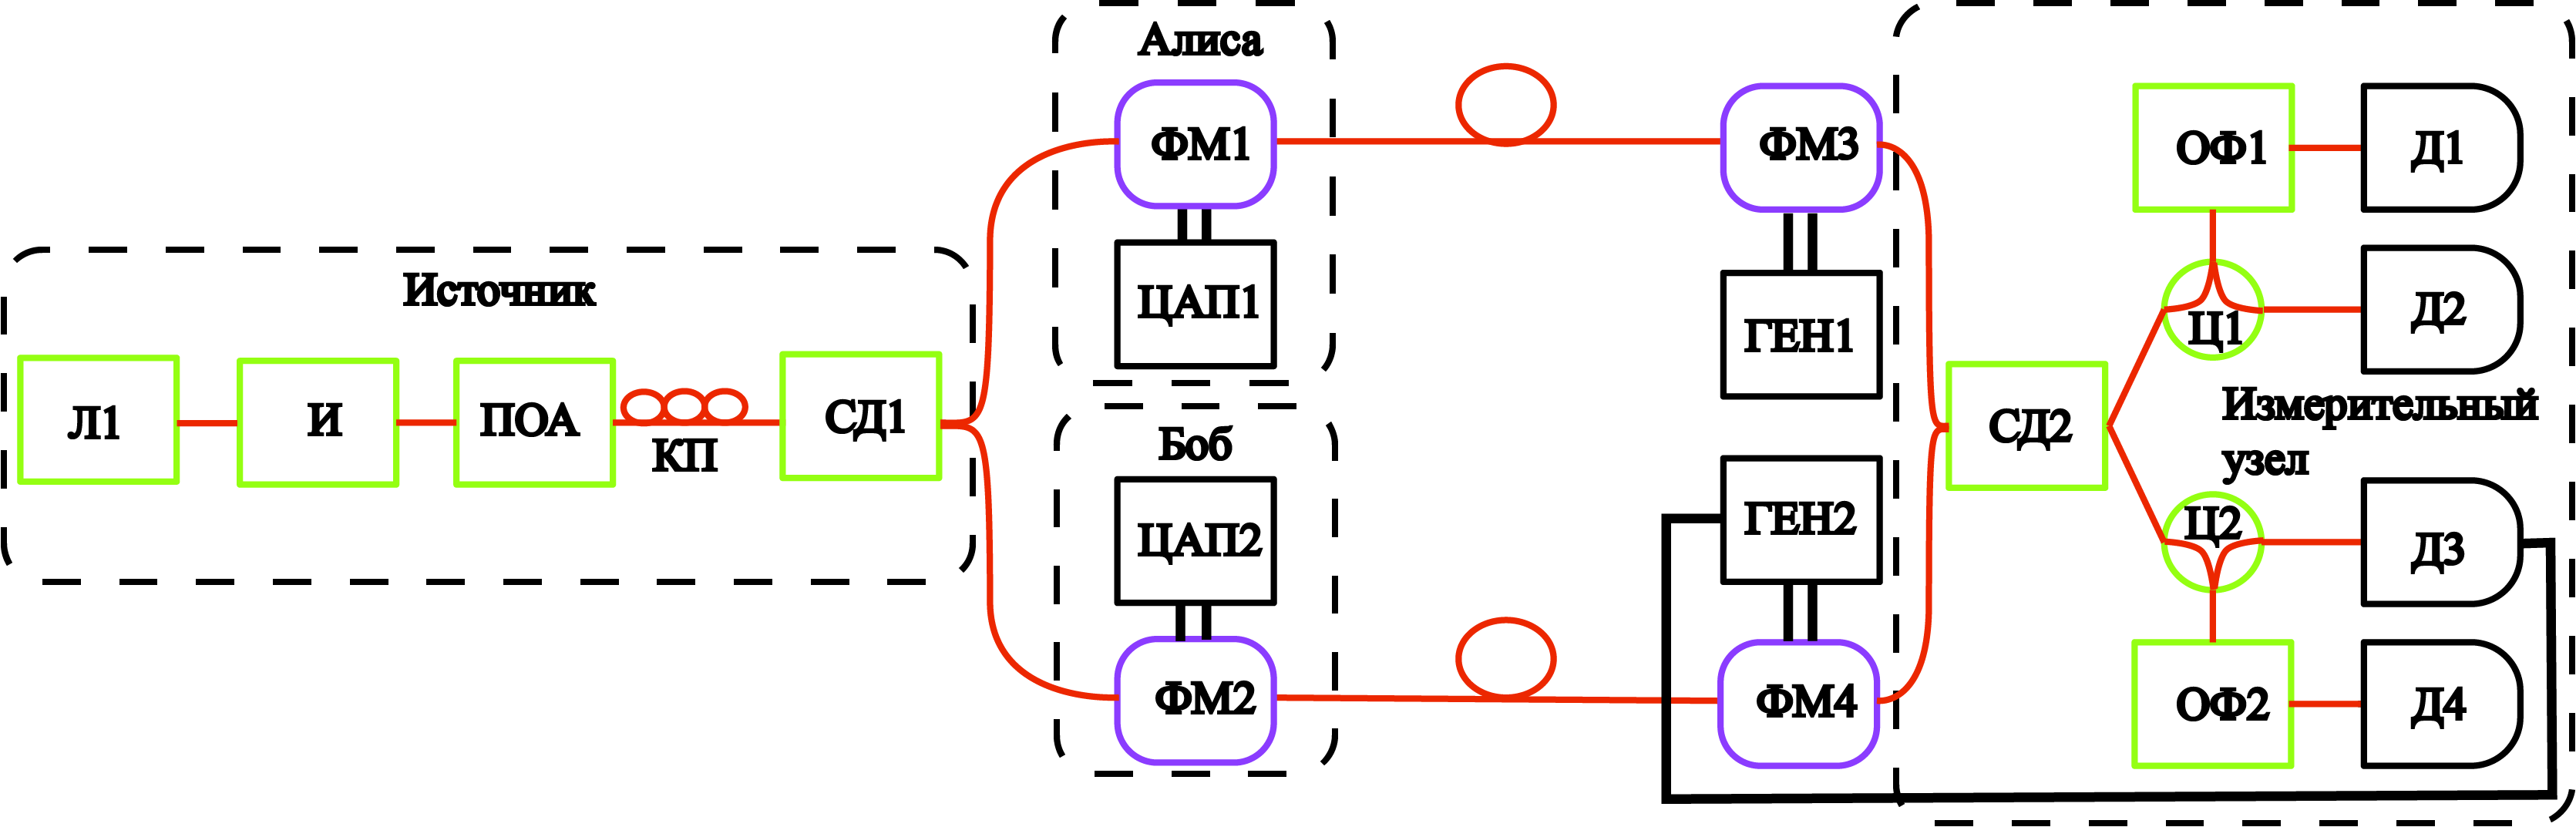
\includegraphics[scale=0.4]{Scheme_colored_rus.png}
  \caption{Experimental setup scheme}
  \label{fig:RF_sin}
\end{figure}

  
 
  
At the output of the source, the signal passed along the two arms of the beam splitter, simulating Alice and Bob as separate nodes. In each node the information was encoded using phase modulators. The outputs of the first beam splitter were connected to the inputs of two independent 10~GHz electro-optical modulators based on $LiNbO_3$ (with built-in polarizer) $PM1$ and $PM2$. Two polarizers reduced the sensitivity of modulators to polarization state of the input light beam. A polarization controller (PC) was used to increase the visibility of the interference pattern. Electrical inputs of $PM1$ and $PM2$ were connected to the outputs of digital-to-analog converters (DAC) applying modulating sinusoidal radio signal with frequency 4.8~GHz. The amplitudes of the control signals were selected so that the signal power at the side frequencies of Alice and Bob would be equal.

The modulation index, which denotes the fraction of energy at the sidebands relative to the central frequency as a result of modulation, should be equal to 5~\%. In this case optimal signal to noise ratio is observed. So the average optical power in the quantum channel was 2.56~pW, which corresponds to $\mu=0.2$.  


In this study we used only two phase states on Alice and Bob ($\varphi_{A,B}\in\{0,\pi\}$. Phase difference ($\Delta\varphi$) between Alice and Bob was formed by changing the IQ tables of the DACs using FPGAs and external software. In case of measuring the dependence of the number of detectors clicks on phase difference ($\Delta\varphi$) the phase was shifted sequentially with a step $\varphi_{step}\ = 10^{\circ}$. Signals on $PM1$ and $PM2$ outputs can be described as shown in ~\ref{phi}.

After the states are prepared, we send them to the quantum channel. To compensate the optical path difference in the two arms of the interferometer, as well as to fine tune the optical phases of the signals, $PM3$ and $PM4$ were used. This adjustment was carried out by changing the DC voltage supplied to the modulators and generated by two independent electrical outputs of the signal generators $GEN1$ and $GEN2$. The outputs of the second pair of phase modulators were connected to a pair of input ports of the 2:2 beam splitter $BS2$ with a splitting ratio of 50:50.

The measurements were carried out in two stages: firstly in classical light, and on the second stage in the photon-counting mode on a superconducting single-photon detector (Scontel), into which two independent receivers $D1$ and $D4$ are built-in. The quantum efficiency of both was 10~\%, and the level of dark counts did not exceed 50~Hz for each. The measured total noise value, including dark counts and parasite illumination from the center frequency due to limited optical filter extinction, was $\gamma_{dark} = 1.5$ kHz.

We demonstrated the dependencies of sidebands intensity after interference on phase difference between the modulating signals in the classical and photon-counting modes. We have also estimated the main parameters characterizing QCS: quantum bit error rate (QBER) and the average sifted key generation rate $ K $, that corresponds to information that is shared by the legitimate users, but possibly correlates with the eavesdropper, therefore requiring privacy amplification procedure to generate a secret quantum key.



 \underline{\textbf{Conclusion}} contains the list of main results. 

% !_____!
  %% Согласно ГОСТ Р 7.0.11-2011:
%% 5.3.3 В заключении диссертации излагают итоги выполненного исследования, рекомендации, перспективы дальнейшей разработки темы.
%% 9.2.3 В заключении автореферата диссертации излагают итоги данного исследования, рекомендации и перспективы дальнейшей разработки темы.
\begin{enumerate}
  \item На основе экспериментального анализа детектора, работающего в режиме Гейгера, показано, что требуются дополнительные средства защиты от атаки с выведением из режима Гейгера при помощи коротких оптических импульсов с энергией не менее 15,4 фДж и при постоянном уровне оптической засветки средним уровнем мощности излучения не менее 35 нВт. 
  \item Численные исследования показали, что измерение величины оптического излучения на несущей частоте, отраженного от оптического фильтра, при помощи мониторного фотодиода в приемном блоке системы квантовой коммуникации на боковых частотах в диапазоне от 7 нВт до 2,93 мкВт с применением дополнительных мер в виде пассивного оптического аттенюатора номиналом 10 дБ для его защиты позволяет противостоять атаке с выведением детектора одиночных фотонов из режима Гейгера и навязыванием ключа нелегитимным пользователем. 
  \item Метод квантовой коммуникации на боковых частотах позволяет реализовывать протокол, устойчивый к контролю нелегитимным пользователем измерительного оборудования.
  \item Для выполнения поставленных задач был создан экспериментальный стенд и в результате интерференции квантового фазомодулированного сигнала на боковых частотах на симметричном светоделителе в схеме квантовой рассылки ключа с узлом регистрации, независящим от легитимного пользователя, наблюдается спектральное разделение квантового сигнала и сигнала на центральной длине волны с их независимой регистрацией в разных плечах светоделителя. 
\end{enumerate}

%	\newcommand{\publications}{\underline{\textbf{\publicationsTXT}}}

{The main results of the dissertation are listed in following publications, included in Scopus and Web of Science:}
\begin{enumerate}\addtolength{\itemsep}{-0.5\baselineskip}
\renewcommand{\labelenumi}{[\theenumi]}
\item Vladimir Chistiakov, Anqi Huang, Vladimir Egorov, and Vadim Makarov, Controlling single-photon detector ID210 with bright light, Opt. Express 27, 32253-32262 (2019)
\\
\item Чистяков В.В., Гайдаш А.А., Козубов А.В., Глейм А.В. Исследование интерференции слабых когерентных многомодовых состояний для задач квантовой коммуникации с недоверенным приемным узлом // Научно-технический вестник информационных технологий, механики и оптики. 2019. Т. 19. № 6. doi: 10.17586/2226-1494-2019-19-6
\\
\item    Gleim A.V., Egorov V.I., Nazarov Y.V., Smirnov S.V., Chistyakov V.V., Bannik O.I., Anisimov A.A., Kynev S.M., Ivanova A.E., Collins R.J., Kozlov S.A., Buller G. Secure polarization-independent subcarrier quantum key distribution in optical fiber channel using BB84 protocol with a strong reference//Optics express, IET - 2016, Vol. 24, No. 3, pp. 2619-2633
\\
\item  Глейм А.В., Егоров В.И., Чистяков В.В., Смирнов С.В., Банник О.И., Булдаков Н.В., Гайдаш А.А., Козубов А.В., Васильев А.Б., Кынев С.М., Хоружников С.Э., Козлов С.А., Васильев В.Н. Квантовая коммуникация на боковых частотах со скоростью 1 Мбит/с в городской сети // Оптический журнал -2017. - Т. 84. - № 6. - С. 3-9
\\
\item  Chistyakov V.V., Kynev S.M, Smirnov S.V., Nazarov Y.V., Gleim A.V. Achieving high visibility in subcarrier wave quantum key distribution system // Journal of Physics: Conference Series, IET - 2016, Vol. 735, No. 1, pp. 012085
\\
\item V. V. Chistyakov, A. V. Gleim, V. I. Egorov, Yu. V. Nazarov. Implementation of multiplexing in a subcarrier-wave quantum cryptography system // Journal of Physics: Conference Series - 2014  vol. 541,  pp. 012078
\\
\item   Kynev S.M., Chistyakov V.V., Smirnov S.V., Volkova K.P., Egorov V.I., Gleim A.V. Free-space subcarrier wave quantum communication // Journal of Physics: Conference Series - 2017, Vol. 917, No. 5, pp. 052003
\\

\item    Gleim A.V., Nazarov Y.V., Egorov V.I., Smirnov S.V., Bannik O.I., Chistyakov V.V., Kynev S.M., Anisimov A.A., Kozlov S.A., Vasil'ev V.N. Subcarrier Wave Quantum Key Distribution in Telecommunication Network with Bitrate 800 kbit/s//EPJ Web of Conferences, IET - 2015, Vol. 103, pp. 10005
\\
\item    Gleim A.V., Egorov V.I., Nazarov Y.V., Smirnov S.V., Chistyakov V.V., Bannik O.I., Anisimov A.A., Kynev S.M., Collins R.J., Kozlov S.A., Buller G.S. Polarization insensitive 100 MHz clock subcarrier quantum key distribution over a 45 dB loss optical fiber channel // Conference on Lasers and Electro-Optics, CLEO 2015, IET - 2015, pp. 7182997
\\
\item Gaidash A.A., Kozubov A.V., Chistyakov V.V., Miroshnichenko G.P., Egorov V.I., Gleim A.V. Security conditions for sub-carrier wave quantum key distribution protocol in errorless channel // Journal of Physics: Conference Series - 2017, Vol. 917, No. 6, pp. 062014
\\
%\item  Gleim A.V., Chistyakov V.V., Bannik O.I., Egorov V.I., Buldakov N.V., Vasilev A.B., Gaidash A.A., Kozubov A.V., Smirnov S.V., Kynev S.M., Khoruzhnikov S.E., Kozlov S.A., Vasil'ev V.N. Sideband quantum communication at 1 Mbit/s on a metropolitan area network // Journal of Optical Technology - 2017, Vol. 84, No. 6, pp. 362-36
\\

\end{enumerate}
\noindent{Other publications:}
\begin{enumerate}\addtolength{\itemsep}{-0.5\baselineskip}
\renewcommand{\labelenumi}{[\theenumi]}
\setcounter{enumi}{9}
\item   Чистяков В.В., Кынев С.М., Смирнов С.В., Назаров Ю.В., Глейм А.В. Обеспечение высокой видности в системе квантовой криптографии на боковых частотах // Сборник трудов IX международной конференции молодых ученых и специалистов «Оптика – 2015», с. 658-660
\\
\item Глейм А.В., Назаров Ю.В., Егоров В.И., Чистяков В.В, Смирнов С.В., Банник О.И., Кынев С.М., Иванова А.Е., Дубровская В.Д., Тарасов М.Г., Булдаков Н.В., Кузьмина Т.Б., Чивилихин С.А., Анисимов А.А., Рощупкин С.В., Рогачёв К.С., Хоружников С.Э., Козлов С.А., Васильев В.Н. Создание квантовой сети университета ИТМО //Сборник трудов VIII международной конференции «Фундаментальные проблемы оптики – 2014». Санкт-Петербург, 20-24 октября ,2014, С.3-4,  541 с. 
\\
\item А.В. Глейм, В.И.Егоров, А.А. Анисимов, Ю.В. Назаров, С.М. Кынев, А.В. Рупасов, В.В. Чистяков, А.А.Гайдаш, М.А. Смирнов, С.А. Чивилихин, С.А. Козлов Квантовая рассылка криптографического ключа по оптическому волокну телекоммуникационного стандарта на расстояние 200 км со скоростью 0.18 кбит/с // Cборник трудов III Всероссийская конференция по фотонике и информационной оптике Москва, НИЯУ МИФИ, 2014 с. 17-19
\\


\end{enumerate}


%При использовании пакета \verb!biblatex! список публикаций автора по теме
%диссертации формируется в разделе <<\publications>>\ файла
%\verb!../common/characteristic.tex!  при помощи команды \verb!\nocite!

\ifdefmacro{\microtypesetup}{\microtypesetup{protrusion=false}}{} % не рекомендуется применять пакет микротипографики к автоматически генерируемому списку литературы
\ifnumequal{\value{bibliosel}}{0}{% Встроенная реализация с загрузкой файла через движок bibtex8
  \renewcommand{\bibname}{\large \authorbibtitle}
  \nocite{*}
  \insertbiblioauthor           % Подключаем Bib-базы
  %\insertbiblioother   % !!! bibtex не умеет работать с несколькими библиографиями !!!
}{% Реализация пакетом biblatex через движок biber
  \ifnumgreater{\value{usefootcite}}{0}{
%  \nocite{*} % Невидимая цитата всех работ, позволит вывести все работы автора
  \insertbiblioauthorcited      % Вывод процитированных в автореферате работ автора
  }{
  \insertbiblioauthor           % Вывод всех работ автора
%  \insertbiblioauthorgrouped    % Вывод всех работ автора, сгруппированных по источникам
%  \insertbiblioauthorimportant  % Вывод наиболее значимых работ автора (определяется в файле characteristic во второй section)
  \insertbiblioother            % Вывод списка литературы, на которую ссылались в тексте автореферата
  }
}
\ifdefmacro{\microtypesetup}{\microtypesetup{protrusion=true}}{}
